\chapter{自修复实验系统设计}
为验证本文算法的有效性和可行性。本章设计了一套切实可行的试验系统,并在改系统下成功进行了同步性改善全局最优自修复实验。

\section{系统需求}
在设计系统之前需要明确系统都需要哪些功能。根据前文对自修复算法的描述和分析可知,首先需要有多个机器人实体来完成编队控制和算法执行。实验中为使得多机器人能够保持编队并顺利执行修复动作,机器人必须知道自身的位置,以及邻居机器人的位置信息。因此该系统需要获取机器人的位置信息。当编队中机器人出现缺失时,其邻居机器人要能够判断出邻居的丢失。在梯度扩散与修复状态传递的过程中还需要编队机器人内部的信息通信。另外对于系统的运行与停止需要我们人为的控制,而多个机器人无法手动同时开启或停止,所以需要设计一个远程控制平台来对整个编队进行控制,同时还能够检测编队中各个机器人的转态。本章实验系统主要围绕以上功能需求而设计。

\section{系统框架及组成}
根据以上需求可知,本实验系统主要具备3大功能部分:定位系统、机器人个体控制及通信系统、远程控制系统。图\ref{fig:system_structure}描述了整个系统的框架图,下面依次介绍3个子系统的设计。
\begin{figure}[!htbp]
	\centering
	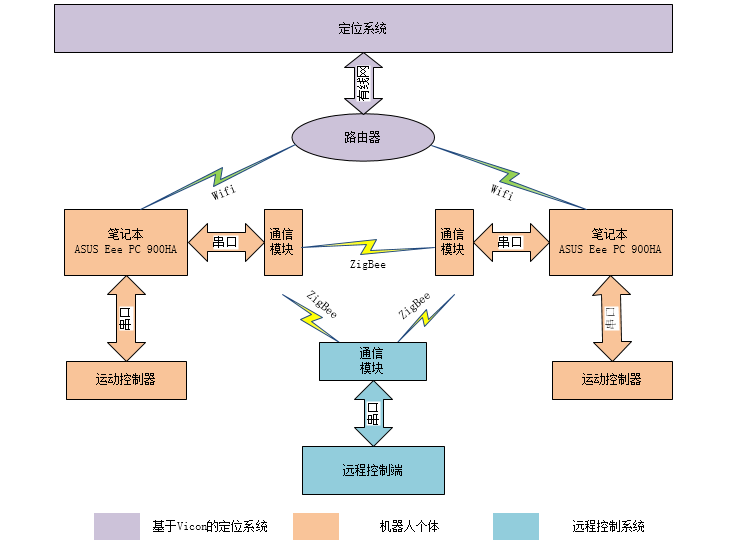
\includegraphics[width=10cm,height=8cm]{chapter4/figure4-3.png}
	\bicaption[fig:system_structure]{试验系统框架示意图}{试验系统框架示意图}{Fig}{The schematic diagram of experimental system.}
\end{figure}

\subsection{定位系统}
本实验系统的定位系统主要采用Vicon光学运动捕捉系统进行机器人的空间定位。Vicon光学运动捕捉系统是由世界上一家非常著名的光学动作捕捉(Motion Capture)系统供应商英国Oxford Metrics Limited 公司生产。它的这项技术在70年代服务于英国海军,从事遥感、测控技术设备的研究与生产。进入80年代他们将自己在军事领域里的高新技术逐渐用于民用方面,在医疗、运动、工程、生物等诸多领域生产制造用于运动捕捉的Motion Capture系统。80年代末,OML公司又将动作捕捉系统技术应用于影视的动画制作领域。
\begin{figure}[!htbp]
	\centering
	\subfigure[运动捕捉系统]{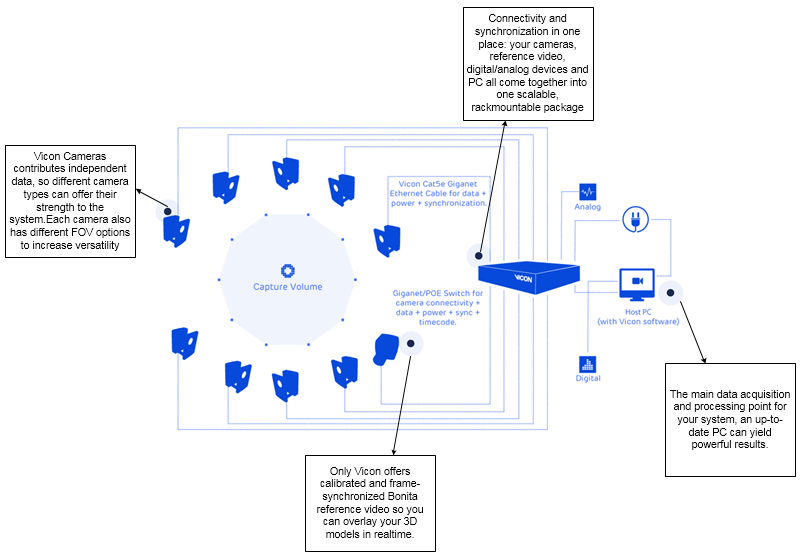
\includegraphics[width=8cm,height=6cm]{chapter4/figure4-1a.png}}
	\subfigure[Vicon 摄像头]{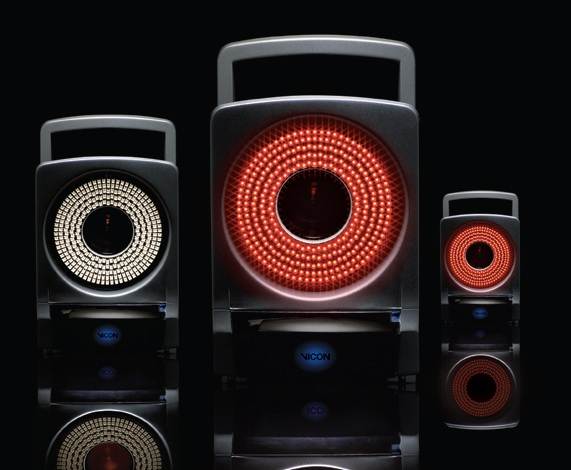
\includegraphics[width=5cm,height=4cm]{chapter4/figure4-1b.jpg}}
	\bicaption[fig:vicon_camera]{Vicon光学运动捕捉系统示意图}{Vicon光学运动捕捉系统}{Fig}{The Vicon motion capture system.}
\end{figure}

Vicon 是英国 OML 公司生产的光学动作捕捉 motion capture 系统。它是世界上第一个设计用于运动捕捉的光学系统,它以自己非凡的技术性能在 motion capture 系统硬件制造领域赢得了极高的声誉,并且改写了 motion capture 系统传统意义上涵盖的内容。它由一组网络连接的 Vicon MX 运动捕捉摄像机和其它设备,建立起一个完整的三维运动捕获系统,以提供实时光学数据,这些数据可以被应用于实时在线或者离线的运动捕捉、分析,应用领域涉及动画制作、虚拟现实系统、机器人遥控、互动式游戏、体育训练、人体工程学研究、生物力学研究等方面。

Vicon运动捕捉系统的主要功能为:

Vicon 系统是非常准确和可靠的光学动作捕捉系统,它所提供的实时光学数据,可以被应用于实时在线或者离线的运动捕捉、分析。

特点:\\
\indent 1)Vicon 公司开发了自己专利的 Vicon Vegas 传感器,可以实现高分辨率与高捕捉频率的同时性,实时捕捉三维效果好,功能强。\\
\indent 2)MX Control 提供 Vicon MX 系统与第三方设备之间的接口,包括测力板、肌电设备、音频、数据手套、眼球跟踪器或者其它数字设备,也可以包含其它附加的板卡以增强 Vicon MX 系统的功能。\\
\indent 3)捕捉摄像机精度高,得到数据非常稳定,捕捉距离也更远。\\
\indent 4)局部捕捉标记点即使被身体挡住,经过软件处理后仍然可以得到令人满意的输出数据。\\
\indent 5)MX 系统安装、调试方便,脱离了旧系统的数据服务器,运输携带更方便。\\
\indent 6)软件界面人性化,数据处理能力强,批处理功能十分方便。

如此高性能的运动捕捉设备,配合Vicon的应用软件Tracker3可以实现高精度,低延迟,多目标的机器人空间定位系统。结合Tracker3应用软件,系统具有如下性能特点:\\
\indent 1)摄像头越多可追踪目标数越多。最低延迟可达到2.8ms处理10个目标,1.9ms处理5个目标。\\
\indent 2)数据从观测端到使用端5ms低延迟。\\
\indent 3)集成实时数据引擎,可以为第三方应用提供数据流,并支持单播TCP链接和多播UDP链接。\\
\indent 4)结合Vicon DataStream SDK 接口,支持 C++, .NET, Windows, Linux, ROS等,方便开发。\\
\indent 5)记录原始数据,支持回放以及离线数据分析。

为使如此高性能的设备充分发挥价值,在定位系统设计时就需要考虑开发的可扩展性,以及功能的丰富性。

\subsection{机器人个体控制及通信系统}
本实验系统机器人个体采用本实验室自主研发的Frontier \uppercase\expandafter{\romannumeral3} 型自主移动机器人平台,如图\ref{fig:robot_zigbee}(a)所示。小车上搭载ASUS Eee PC 900HA笔记本电脑作为控制中心,分布式自修复算法运行在此笔记本之上。笔记本通过串口向小车的运动控制器发送速度信息从而控制小车运动。小车上安装有反光球用于运动捕捉系统的识别与定位。
\begin{figure*}[!htbp]
	\centering
	\subfigure[机器人个体]{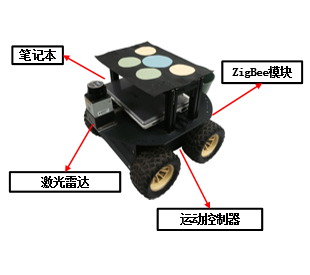
\includegraphics[width=5cm,height=4cm]{chapter4/figure4-2a.png}}
	\hspace{1cm}
	\subfigure[ZigBee通信模块]{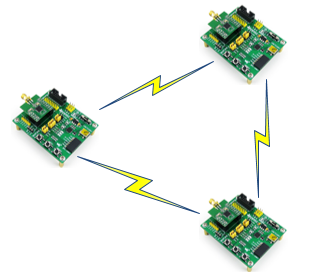
\includegraphics[width=5cm,height=4cm]{chapter4/figure4-2b.png}}
	\bicaption[fig:robot_zigbee]{机器人个体与ZigBee通信模块}{机器人个体与ZigBee通信模块}{Fig}{The robot and ZigBee communication model.}
\end{figure*}

在本系统中包含有多种方向的通信,包括定位系统与机器人之间的通信,远程控制系统与机器人之间的通信,机器人与机器人之间的通信。其中,定位系统与机器人之间的通信采用局域网内部的网络通信方式。而机器人之间的通信由于需要多对多通信,且通信频繁数据量小,再有通信拓扑在算法执行过程中会动态建立以及切换,所以采用ZigBee作为机器人之间的组网通信方式,如图\ref{fig:robot_zigbee}(b)所示。ZigBee通信网络具有低功耗、低成本、近距离、短时延、高安全、工作频段灵活等特性。另外,主要是ZigBee的自组网通信方式可以轻松满足K邻居拓扑网络的构建与拓扑切换的需求。

\subsection{远程控制系统}
远程控制系统主要是为实现对编队机器人同时控制,且显示各个机器人状态信息。远程控制的实现主要通过ZigBee网络中的协调器对所有编队机器人进行广播。

\section{系统设计}

\subsection{定位系统}
鉴于Vicon光学运动捕捉系统的强大功能,本系统的设计不只考虑用于多机器人编队自修复的定位需求,同时考虑本实验室的多种机器人如无人机、机械臂,软体手术机器人的空间定位需求而开发。另外在设计过程中充分考虑了功能的可扩展性,方便以后机器人种类的增加或者功能的变化。在几种机器人当中根据结构可以大致分为两类,一种是刚体机器人,如本实验所需的小车,无人机,机械臂。另一种是柔性机器人,如软体手术机器人。针对这两类需求,Vicon运动捕捉系统提供了两款应用软件Tracker和Nexus。在这两款软件上可以对Vicon摄像头进行命名、参数配置和调整、标定、目标选择与命名等操作。然而这两款软件无法满足某些特定应用场景的需求,因此本文介绍的系统是在Vicon官方开放的sdk基础上进行的二次开发以满足本实验系统以及其他特定种类机器人的需求。本文定位系统设计的主要工作是开发了一款服务器端软件,软件集成了空间机器人的数据采集,分析,封装,转发,显示,存储等功能。开发环境为\textbf{Windows7}操作系统下的\textbf{visual studio 2013}编辑器,采用\textbf{MFC}框架。

对于刚体结构的机器人和柔性结构的机器人Tracker和Nexus提供的数据形式不同,因此针对两类需求分别设计了不同的数据处理方式以及UI显示界面。在程序启动时需要根据具体需求选择不同的应用模式,如图\ref{fig:select_mode}所示,软件分为ViconSystem\_Nexus模式和ViconSystem\_Tracker模式,分别针对Nexus软件和Tracker软件使用。
\begin{figure}[!htbp]
	\centering
	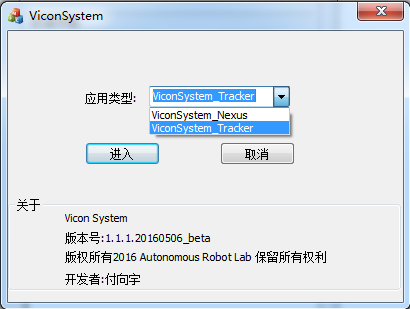
\includegraphics[width=8cm,height=5.5cm]{chapter4/figure4-4.png}
	\bicaption[fig:select_mode]{软件模式选择}{软件模式选择}{Fig}{Selection of software mode.}
\end{figure}

目前,由于ViconSystem\_Nexus模式下除软件的数据处理方式与部分UI界面与ViconSystem\_Tracker不同外其他功能类似,且数据种类不如ViconSystem\_Tracker模式下丰富。因此下文主要根据ViconSystem\_Tracker模式的软件开发进行介绍。

图\ref{fig:software_diagram}描述了定位系统的软件结构层次。不同层对应系统不同部分。
\begin{figure}[!htbp]
	\centering
	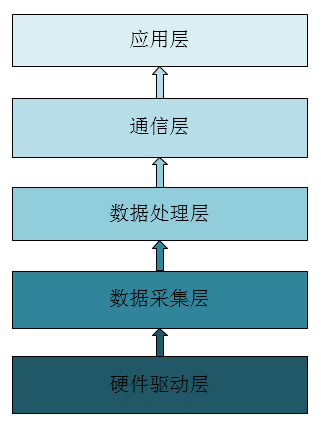
\includegraphics[width=4cm,height=6cm]{chapter4/figure4-5.png}
	\bicaption[fig:software_diagram]{软件结构层次图}{软件结构层次图}{Fig}{Software structure level diagram.}	
\end{figure}

\indent \textbf{硬件驱动层与数据采集层:}这两层对应Vicon运动捕捉系统的硬件设施与Tracker应用软件。Vicon系统服务器驱动10台运动捕捉相机,对相机进行标定之后,在Tracker软件中根据识别的反光球标记机器人并命名。运动捕捉相机将采集的数据上传到数据中心,在数据中心中对相机数据进行处理,计算出空间中各个机器人的位姿信息。\\
\indent \textbf{数据处理层与通信层:}本文所开发的软件主要是属于这两层。软件通过sdk提供的接口将数据中心计算的位姿信息获取到,然后进一步对数据进行处理,显示、存储、以及封装成应用层需要的数据形式。在通信层将封装好的数据通过局域网内的wifi传输给应用层。\\
\indent \textbf{应用层:}这一层主要对应机器人,如何使用数据取决于机器人要实现的功能。

图\ref{fig:flow_chart}是程序设计的流程图,程序采用多线程设计,主要分为数据采集与处理线程和数据传输线程,在两个线程之间存在数据同步。
\begin{figure}[!htbp]
	\centering
	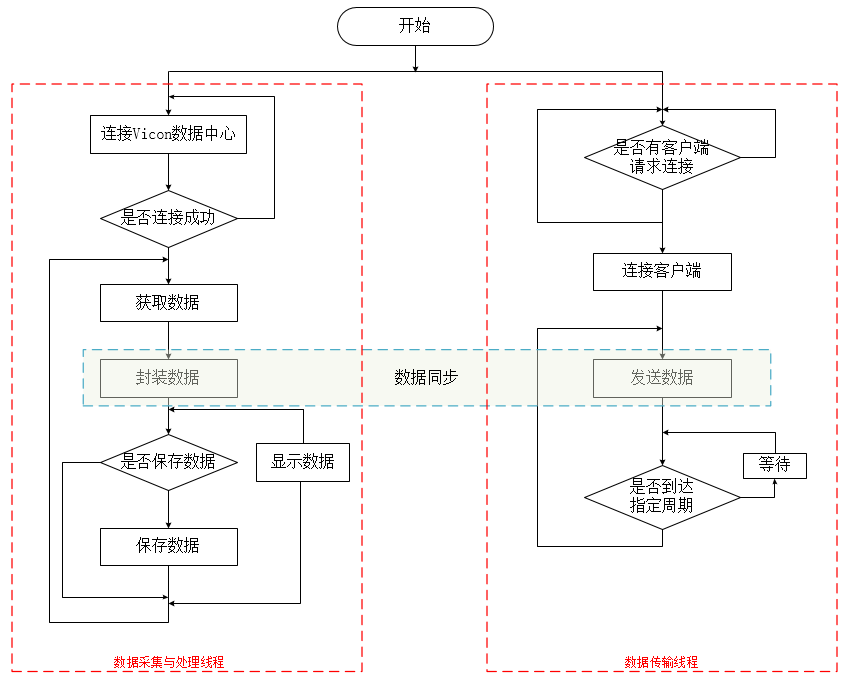
\includegraphics[width=8cm,height=7cm]{chapter4/FlowChart.png}
	\bicaption[fig:flow_chart]{定位系统程序设计流程图}{定位系统程序设计流程图}{Fig}{The program flow chart of positioning system software.}
\end{figure}

图\ref{fig:software_ui}是软件的用户界面。
\begin{figure}[!htbp]
	\centering
	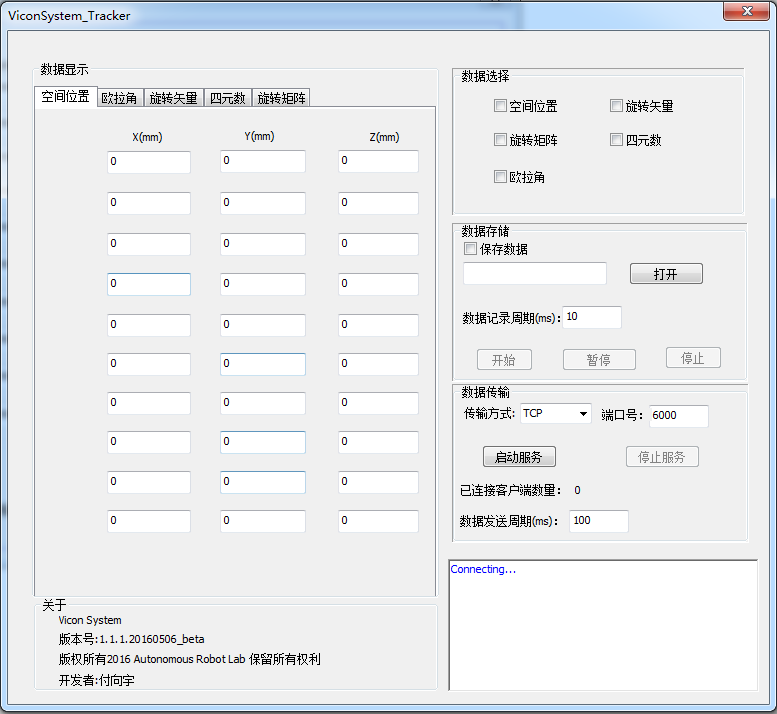
\includegraphics[width=10cm,height=8cm]{chapter4/figure4-6.png}
	\bicaption[fig:software_ui]{定位系统ViconSystem\_Tracker模式软件界面}{定位系统ViconSystem\_Tracker模式软件界面}{Fig}{The user interface of ViconSystem\_Tracker mode.}
\end{figure}

软件实现的主要功能有:\\
\indent 1)实现目标在空间中的位置、旋转矢量、旋转矩阵、四元数、欧拉角等数据的实时采集与显示。\\
\indent 2)支持多客户端链接,并实时发送以上数据到客户端,发送的数据可以按照需求在数据选择框中进行勾选。\\
\indent 3)数据发送方式支持TCP协议和UDP协议。\\
\indent 4)支持发送周期可调(单位ms),系统初始默认周期为100ms。\\
\indent 5)支持数据本地存储,方便离线分析。数据存储的类型与发送给客户端的数据类型同步,都是根据在数据选择框中所勾选的数据进行处理。数据本地记录的周期可调,默认为10ms。

ViconSystem\_Tracker模式主要是针对刚体在空间中的位姿数据获取,每一个刚体需要贴3个以上的反光球。获取到的数据是整个刚体的位姿数据。例如空间位置是刚体上所有反光球位置的平均值。但是考虑柔性结构的机器人,它在空间中会发生形变,因此我们想要得到的数据是柔性结构的每一点的位置数据。ViconSystem\_Nexus即是为此需求而设计,背后依托的是Vicon运动捕捉系统的Nexus软件。在ViconSystem\_Nexus下没有各种不同的位姿数据,只显示每个反光球在空间中的位置数据。其他功能与ViconSystem\_Tracker模式下类似,因此不再具体介绍。软件用户界面如图\ref{fig:software_ui2}所示。
\begin{figure}[!htbp]
	\centering
	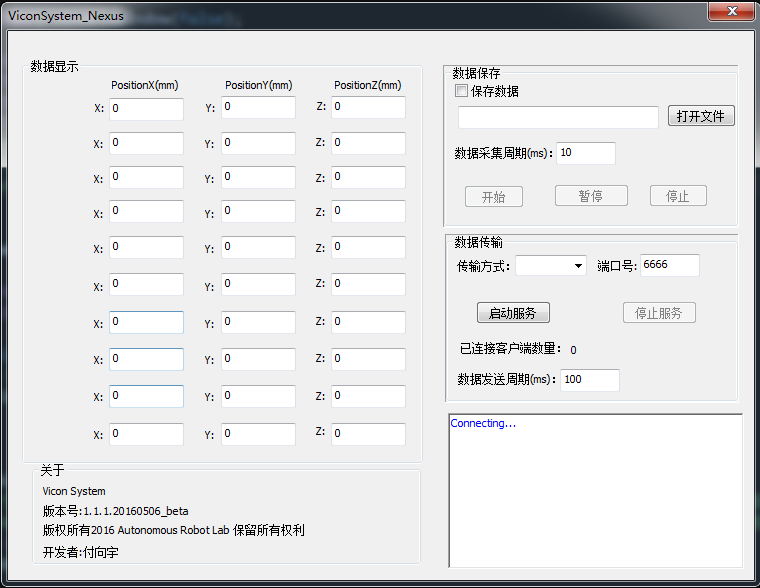
\includegraphics[width=10cm,height=8cm]{chapter4/figure4-7.png}
	\bicaption[fig:software_ui2]{定位系统ViconSystem\_Nexus模式软件界面}{定位系统ViconSystem\_Nexus模式软件界面}{Fig}{The user interface of ViconSystem\_Nexus mode.}
\end{figure}

\subsection{机器人个体与通信系统}
机器人个体控制主要是在ASUS Eee PC 900HA笔记本电脑上实现第3章所描述的自修复算法,开发环境为vc6.0。通过串口向基于DSP实现的运动控制板发送速度命令。利用ZigBee与邻居进行通信,同时通过ZigBee与远程控制端进行交互。图\ref{fig:clientSoftware}是机器人个体控制的用户界面,继承了参数设置,状态显示,运动控制的功能。

\begin{figure}[!htbp]
	\centering
	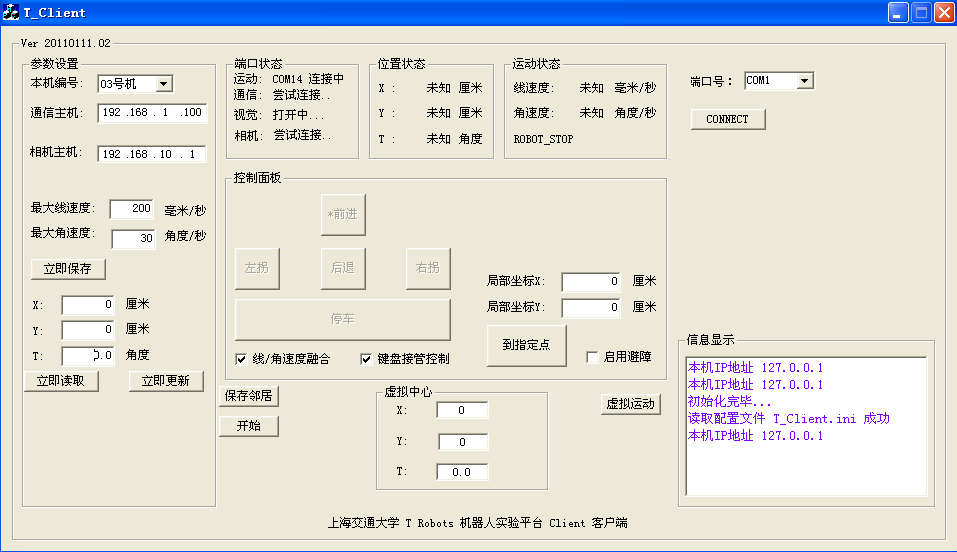
\includegraphics[width=10cm,height=6cm]{chapter4/figure4-8.png}
	\bicaption[fig:clientSoftware]{机器人个体控制的软件用户界面}{机器人个体控制的软件用户界面}{Fig}{The user interface of robot client software.}
\end{figure}

\subsection{远程控制系统}
远程控制系统主要是通过串口连接ZigBee网络的协调器,利用协调器向编队网络发送运动控制指令以及少量数据,同时接受来自所有机器人的状态信息并显示,图\ref{fig:RopSoftware}是远程控制端的用户界面。

\begin{figure}[!htbp]
	\centering
	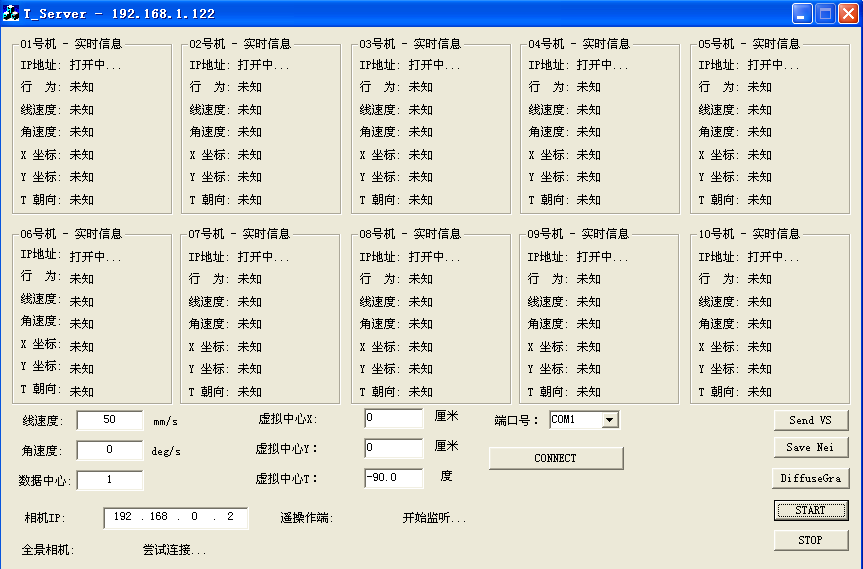
\includegraphics[width=10cm,height=6cm]{chapter4/figure4-9.png}
	\bicaption[fig:RopSoftware]{远程控制系统软件用户界面}{远程控制系统软件用户界面}{Fig}{The user interface of romote operation software.}
\end{figure}

\section{本章小结}
本章介绍了多机器人编队自修复实验平台的设计。实验平台主要包括定位系统,机器人个体控制与通信系统,远程控制系统。其中着重介绍了定位系统的设计,依托Vicon光学运动捕捉系统,设计了功能丰富,适用不同机器人,可扩展的定位系统服务器端软件。机器人个体与通信系统实现了本文的同步性改善全局最优的分布式递归自修复算法。远程控制系统实现对编队的远程统一控制与转态回显。
